%%%%%%%%%%%%%%%%%%%%%%%%%%%%%%%%%%%%%%%%%%%%%%%%%%%%%%%%%%%%%%%%%%%%%%%%%%%
%  TP2 - Compensacion de efectos de transmisor (LTX)
%  Codigo: simulador/  (tx_dpmzm, ltx_compensator, aligner_lanes, fsm_rx)
%  Figuras: simulador/run_tp2_ej2 ... run_tp2_ej6
%%%%%%%%%%%%%%%%%%%%%%%%%%%%%%%%%%%%%%%%%%%%%%%%%%%%%%%%%%%%%%%%%%%%%%%%%%%

\section*{Compensación de efectos de transmisor}

%==========================================================================
\subsection*{Ejercicio 1: Implementación}
%==========================================================================

Se incorporó al simulador del trabajo práctico 1 el transmisor óptico de
doble polarización y, a la salida del lazo principal del receptor, los
compensadores de desbalance I/Q y de skew. Todos los bloques nuevos tienen
un indicador de habilitación: con ellos apagados el simulador reproduce
exactamente los resultados del trabajo práctico 1, lo que se verificó
comparando una corrida con la misma semilla antes y después de los
cambios. La Figura~\ref{fig:ej1_diagrama} muestra el sistema completo.

\begin{figure}[H]
\centering
\begin{tikzpicture}[
    font=\scriptsize,
    blk/.style={draw, rounded corners=2pt, align=center, minimum height=8mm,
                minimum width=14mm, inner sep=2pt, fill=white},
    nuevo/.style={blk, fill=gray!20},
    flecha/.style={-{Stealth[length=1.6mm]}},
    grupo/.style={draw, dashed, rounded corners=4pt, inner sep=5pt},
    node distance=4mm and 3mm]
% ---------------- transmisor ----------------
\node[blk]   (qam)  {QAM\\gen.\\(H y V)};
\node[blk,   right=of qam]  (rrc)  {RRC +\\resampler};
\node[nuevo, right=9mm of rrc]  (imp)  {Desperf.\\LTX\\(lane Q)};
\node[nuevo, right=of imp]  (dac)  {DAC};
\node[nuevo, right=of dac]  (drv)  {Driver\\$\times 4$};
\node[nuevo, right=of drv]  (mzm)  {DP-MZM};
\node[nuevo, above=of mzm]  (las)  {Láser\\ideal};
\node[nuevo, right=of mzm]  (pol)  {Pol. H\\(descarta V)};
\draw[flecha] (qam) -- (rrc);
\draw[flecha] (rrc) -- node[above]{4 lanes} (imp);
\draw[flecha] (imp) -- (dac);
\draw[flecha] (dac) -- (drv);
\draw[flecha] (drv) -- (mzm);
\draw[flecha] (las) -- (mzm);
\draw[flecha] (mzm) -- (pol);
% ---------------- canal ----------------
\node[blk, below=10mm of pol] (ch) {Canal: filtro,\\AWGN y\\portadora};
\draw[flecha] (pol) -- (ch);
% ---------------- receptor ----------------
\node[blk,   left=of ch]   (aaf)  {AAF +\\resampler\\+ AGC};
\node[blk,   left=of aaf]  (ffe)  {FFE};
\node[blk,   left=of ffe]  (cpr)  {CPR\\(RFD + FCR)};
\node[blk,   left=of cpr]  (cs)   {Alineación\\+ CS};
\node[nuevo, left=of cs]   (iq)   {Desbalance\\I/Q\\($2\times2$)};
\node[nuevo, below=10mm of iq] (sk) {Skew\\(FIR por\\lane)};
\node[nuevo, right=of sk]  (ub)   {Sesgo\\MMSE +\\slicer};
\node[nuevo, right=of ub]  (al2)  {Alineación 2\\(por lane)};
\node[blk,   right=of al2] (ber)  {BER};
\draw[flecha] (ch)  -- (aaf);
\draw[flecha] (aaf) -- (ffe);
\draw[flecha] (ffe) -- (cpr);
\draw[flecha] (cpr) -- (cs);
\draw[flecha] (cs)  -- (iq);
\draw[flecha] (iq)  -- (sk);
\draw[flecha] (sk)  -- (ub);
\draw[flecha] (ub)  -- (al2);
\draw[flecha] (al2) -- (ber);
% ---------------- grupos ----------------
\begin{scope}[on background layer]
\node[grupo, fit=(qam)(rrc)(imp)(dac)(drv)(mzm)(las)(pol),
      label={[font=\scriptsize]above left:Transmisor DP-MZM}] {};
\node[grupo, fit=(ffe)(cpr),
      label={[font=\scriptsize]above:Lazo principal (TP1)}] {};
\node[grupo, fit=(iq)(sk),
      label={[font=\scriptsize,align=center]left:Compensadores\\del LTX}] {};
\end{scope}
\end{tikzpicture}
\caption{Diagrama en bloques del sistema. En gris, los bloques
incorporados en este trabajo práctico.}
\label{fig:ej1_diagrama}
\end{figure}

\subsubsection*{Transmisor}

El transmisor (\texttt{tx\_dpmzm}) genera dos secuencias 16-QAM, una por
polarización, y las conforma con el mismo filtro RRC del trabajo práctico 1.
A la tasa del canal (4 muestras por símbolo) se separan las cuatro lanes
$H_I$, $H_Q$, $V_I$ y $V_Q$, y cada una recorre la cadena de la
Tabla~\ref{tab:ej1_tx}. Los modelos del driver, del MZM y del láser son
los implementados en el trabajo práctico de óptica, copiados sin cambios
a la carpeta \texttt{simulador/optica}.

\begin{table}[H]
\centering
\small
\begin{tabular}{lll}
\toprule
Bloque & Modelo & Versión ideal \\
\midrule
Desperfectos del LTX & ganancia y retardo de la lane Q & sin desperfectos \\
DAC & escala de tensión ($V_{pp}$ de la forma de onda) & --- \\
Driver & respuesta de 2.º orden, ruido y no linealidad de Rapp & ganancia $G$ \\
Modulador & DP-MZM: senoide, pérdidas, ER y respuesta del MZM & IQ lineal \\
Láser & modelo del TP de óptica & siempre ideal \\
\bottomrule
\end{tabular}
\caption{Cadena de cada lane del transmisor.}
\label{tab:ej1_tx}
\end{table}

Los tres desperfectos del LTX se aplican sobre la lane Q, respecto de la
I:

\begin{itemize}\itemsep2pt
\item Error de ganancia: la lane Q se multiplica por $10^{G_{IQ}/20}$.
\item Skew: la lane Q se retrasa una fracción de símbolo, con un retardo
      fraccionario exacto implementado en frecuencia.
\item Desbalance de fase: se genera con la tensión de bias del
      desfasador de la rama Q, $V_{Bias,\phi} = V_\pi/2 + \Delta\phi\,
      V_\pi/\pi$, de modo que el ángulo entre las ramas es
      $90^\circ + \Delta\phi$.
\end{itemize}

Siguiendo la consigna, a la salida del modulador se descarta la
polarización V y la señal óptica de la polarización H se usa directamente
como señal eléctrica, normalizada a la misma potencia que el transmisor
del trabajo práctico 1.

\subsubsection*{Compensadores}

Los compensadores (\texttt{ltx\_compensator}) operan a un símbolo por
muestra sobre la salida del lazo principal (FFE y recuperación de
portadora), es decir, sobre la señal ya derrotada:
%
\begin{equation}
u \;\rightarrow\; \underbrace{\begin{bmatrix} v_I \\ v_Q \end{bmatrix}
= \mathbf{A}\begin{bmatrix} u_I \\ u_Q \end{bmatrix}}_{\text{desbalance I/Q}}
\;\rightarrow\;
\underbrace{z_I = \mathbf{h}_I^T \mathbf{v}_I,\;\;
z_Q = \mathbf{h}_Q^T \mathbf{v}_Q}_{\text{skew}}
\;\rightarrow\; \text{slicer}.
\end{equation}

\begin{itemize}\itemsep2pt
\item El compensador de desbalance I/Q es una matriz real de $2\times2$
      (un solo tap), inicializada en la identidad.
\item El compensador de skew tiene un FIR real por lane, sin filtros
      cruzados, con cantidad de taps configurable, inicializado en un
      impulso centrado.
\item Ambos se adaptan por LMS dirigido por decisiones, con pasos
      independientes ($\mu_{IQ}$ y $\mu_{sk}$). El de desbalance usa el
      error en su propia salida, en la muestra central del FIR de skew.
\end{itemize}

\paragraph{Arranque ciego del compensador de skew.}
Con skew cercano a $0.5$~UI la lane retrasada se muestrea entre dos
símbolos y vale aproximadamente $c\,(a_n + a_{n+1})$: el ojo está cerrado
(del orden de 10~\% de decisiones erróneas) y los dos símbolos pesan lo
mismo. En esas condiciones el LMS dirigido por decisiones no se mueve de
la identidad, aunque la solución existe: los coeficientes óptimos,
calculados con los símbolos verdaderos, dan $17.6$~dB de SNR con 7 taps
contra $8.1$~dB de la identidad ($E_b/N_0 = 16$~dB). Por eso los primeros
$40\,000$ símbolos de la etapa de skew se adaptan con un criterio ciego
de módulo por lane, $e_I = (R - z_I^2)\,z_I$ con $R =
E\{x^4\}/E\{x^2\}$ de los niveles PAM, y recién después con decisiones.

\paragraph{Alineación 2 por lane.}
Con un skew de un UI o más, el receptor arma puntos válidos de la
constelación con $I(n)$ y $Q(n-k)$: no hay error que ningún algoritmo
dirigido por decisiones pueda detectar, y la alineación del trabajo
práctico 1, que busca un único retardo, falla. La alineación 2
(\texttt{aligner\_lanes}) correlaciona por separado las decisiones de cada
lane con las lanes transmitidas y encuentra para cada una su retardo, su
signo y su correspondencia, lo que cubre el skew entero, la ambigüedad
de $90^\circ$ y la imagen conjugada.

\subsubsection*{Secuencia de la simulación}

La máquina de estados pasa a diez etapas (Tabla~\ref{tab:ej1_fsm}). Los
compensadores del LTX se encienden recién con el lazo principal
convergido y la corrección de cycle slips aplicada, y siguen adaptándose
hasta el final.

\begin{table}[H]
\centering
\small
\begin{tabular}{clcccc}
\toprule
\# & Etapa & Símbolos & FFE & CPR & LTX \\
\midrule
1  & FFE-CMA                  & 60\,000  & CMA & ---      & --- \\
2  & FFE-CMA + RFD            & 50\,000  & CMA & RFD      & --- \\
3  & FFE-CMA + RFD + FCR 4ª   & 30\,000  & CMA & RFD, 4ª  & --- \\
4  & FFE-CMA + FCR-DD         & 20\,000  & CMA & DD       & --- \\
5  & FFE-DD + FCR-DD          & 20\,000  & DD  & DD       & --- \\
6  & Alineación + CS          & 10\,000  & DD  & DD       & --- \\
7  & Desbalance I/Q           & 40\,000  & DD  & DD       & IQ \\
8  & Skew                     & 60\,000  & DD  & DD       & IQ + skew \\
9  & Alineación 2             & 10\,000  & DD  & DD       & IQ + skew \\
10 & Estimación de BER        & variable & DD  & DD       & IQ + skew \\
\bottomrule
\end{tabular}
\caption{Etapas de la máquina de estados del receptor.}
\label{tab:ej1_fsm}
\end{table}

%==========================================================================
\subsection*{Ejercicio 2: Sanidad}
%==========================================================================

\subsubsection*{Curva de BER del caso base}

Se corrió la curva de BER con todos los algoritmos encendidos, incluidos
los dos compensadores nuevos, con canal impulso, transmisor ideal y sin
desperfectos. La penalidad se midió como el corrimiento horizontal de cada
punto respecto de la curva teórica, y se interpoló a $\mathrm{BER} =
10^{-2}$ y $10^{-3}$ (Figuras~\ref{fig:ej2_ber} y~\ref{fig:ej2_pen}).

\begin{figure}[H]
\centering
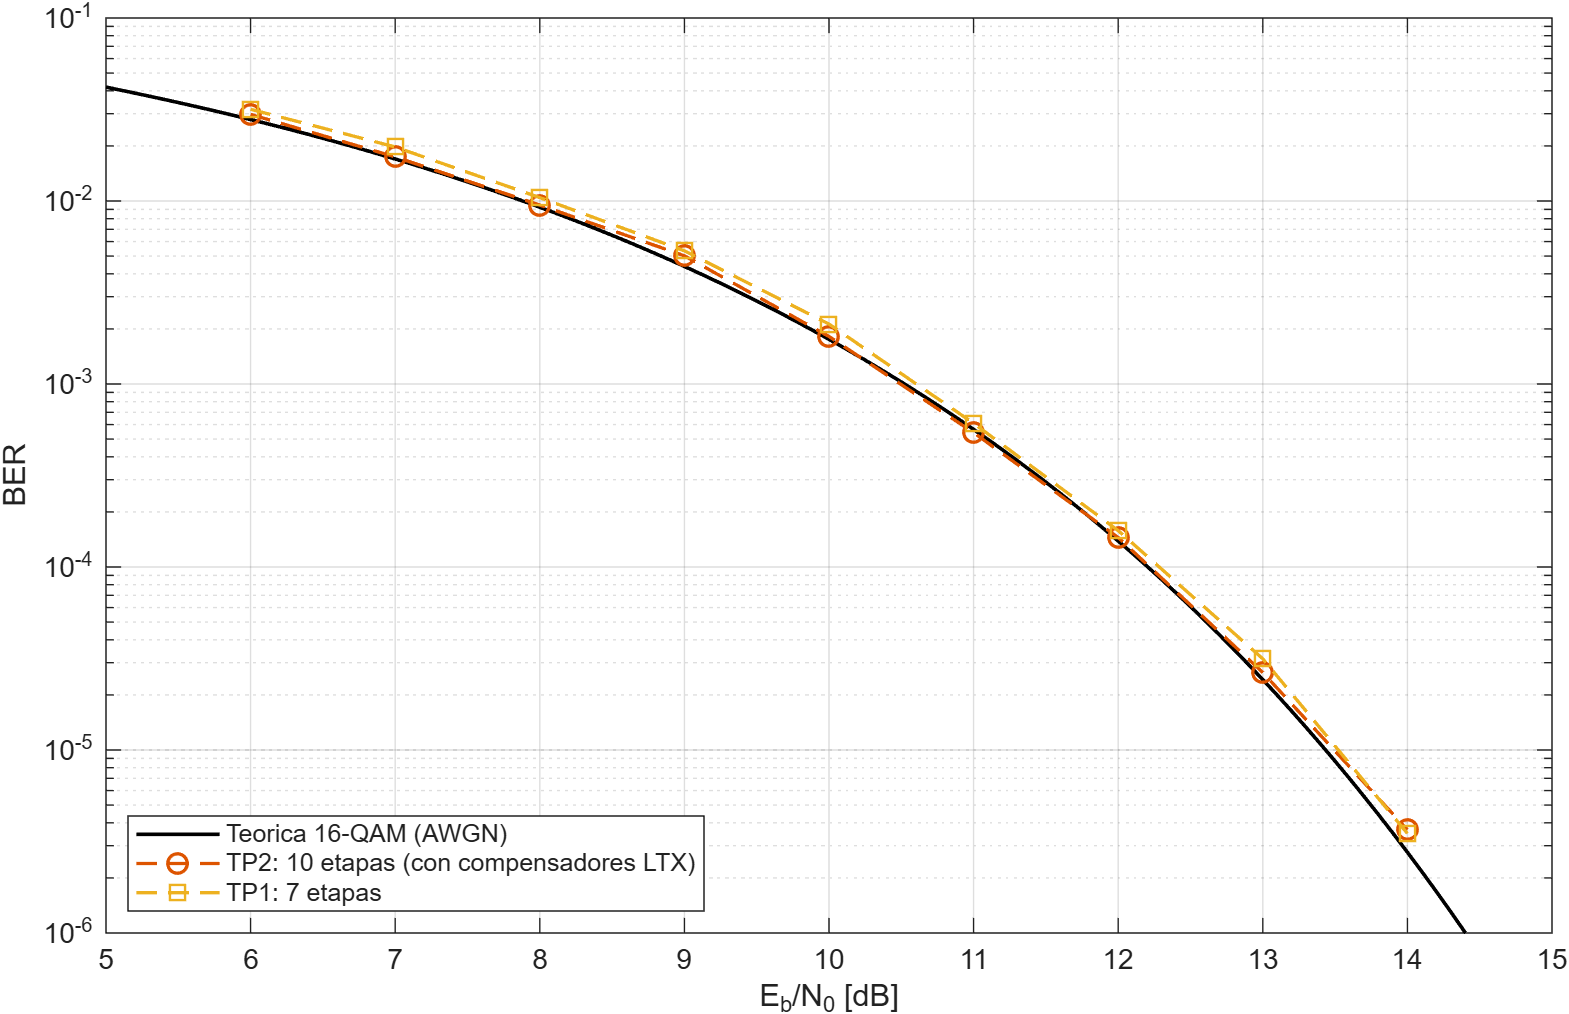
\includegraphics[width=0.75\textwidth]{figuras/ej2_ber_base.png}
\caption{BER del caso base contra la curva teórica de 16-QAM, con el
receptor de diez etapas y con el del trabajo práctico 1.}
\label{fig:ej2_ber}
\end{figure}

\begin{figure}[H]
\centering
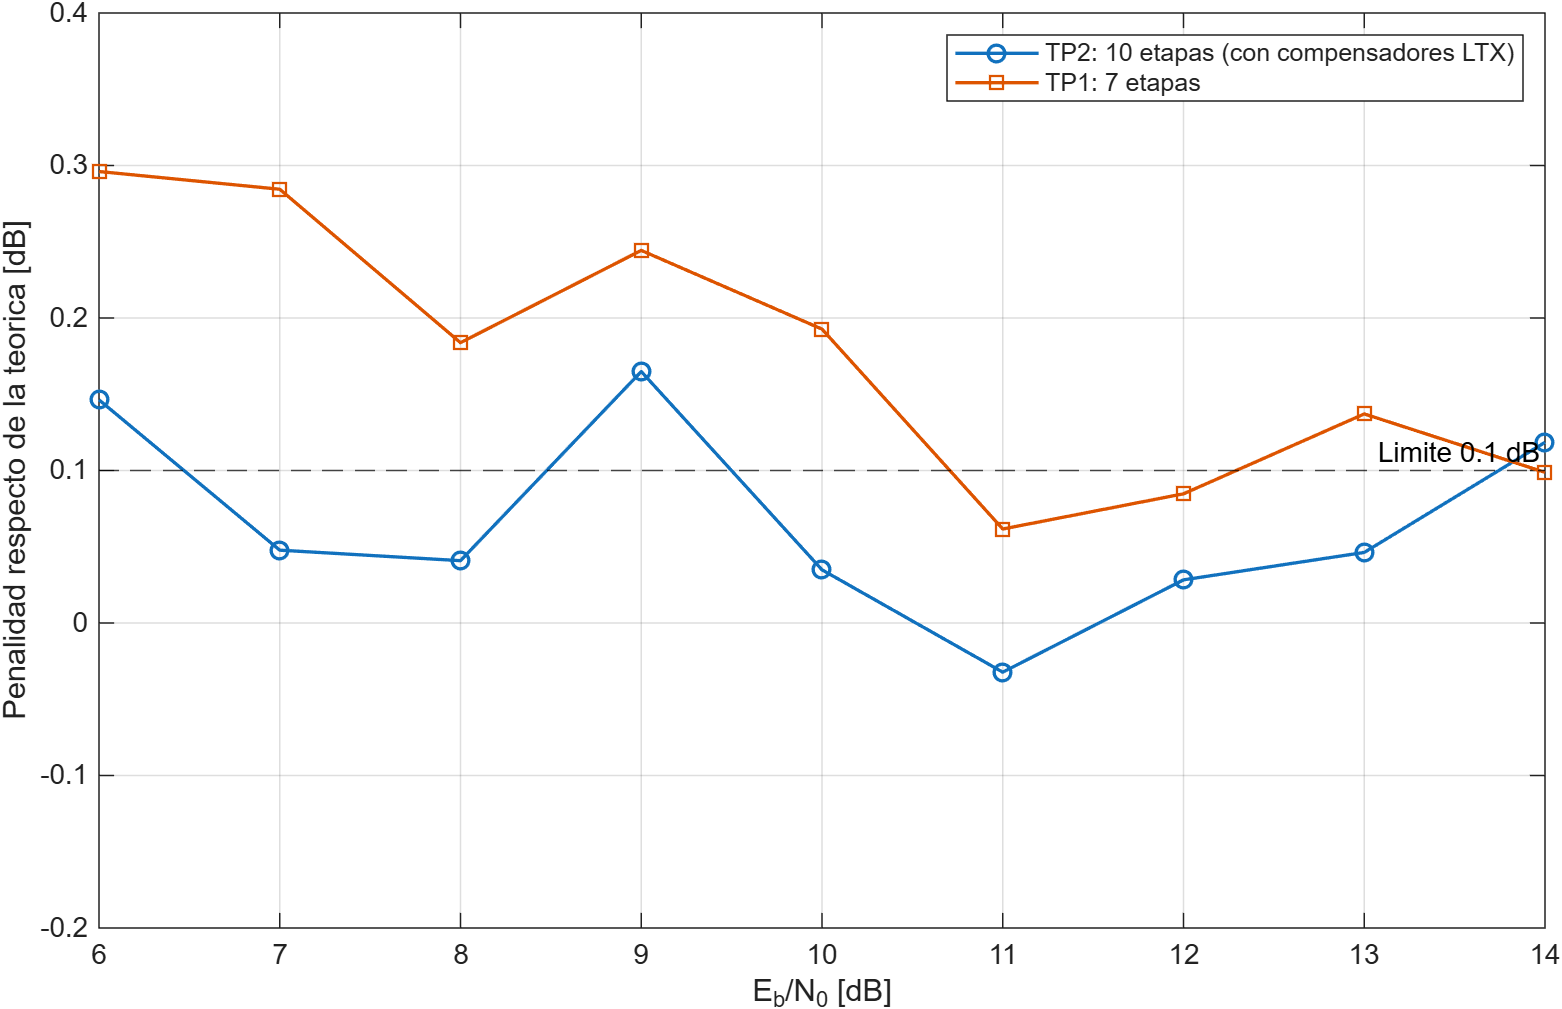
\includegraphics[width=0.7\textwidth]{figuras/ej2_penalidad_base.png}
\caption{Penalidad respecto de la curva teórica en cada punto simulado.}
\label{fig:ej2_pen}
\end{figure}

\begin{table}[H]
\centering
\small
\begin{tabular}{lcc}
\toprule
Receptor & Penalidad @ $10^{-2}$ & Penalidad @ $10^{-3}$ \\
\midrule
10 etapas, con compensadores del LTX & $0.04$~dB & $0.00$~dB \\
7 etapas (trabajo práctico 1)        & $0.19$~dB & $0.11$~dB \\
\bottomrule
\end{tabular}
\caption{Penalidad del caso base.}
\label{tab:ej2_pen}
\end{table}

El caso base cumple el requisito de $0.1$~dB. Para llegar a ese valor se
calibraron:

\begin{itemize}\itemsep2pt
\item Corrección del sesgo MMSE: los LMS dirigidos por decisiones
      convergen a la solución de Wiener, que encoge la constelación. Antes
      del slicer final se estima ese factor contra las propias decisiones
      y se lo divide. Es la principal diferencia con el receptor del
      trabajo práctico 1 en la Tabla~\ref{tab:ej2_pen}.
\item Pasos del FFE en modo DD ($3\times10^{-5}$) y del AGC
      ($10^{-4}$), que reducen el ruido de gradiente.
\item Pasos de los compensadores del LTX: $\mu_{IQ} = \mu_{sk} =
      3\times10^{-4}$. Con $10^{-3}$ el ruido de gradiente sumaba unos
      $0.04$~dB.
\item El detector de frecuencia gruesa (RFD) se acota en los barridos
      sin offset de portadora, igual que en el trabajo práctico 1: sin
      offset su integrador solo acumula ruido.
\end{itemize}

\subsubsection*{Respuesta en frecuencia del driver}

Se habilitó la respuesta lineal del driver, sin ruido ni no linealidad,
con frecuencia natural $0.35\,BR$ y amortiguamiento $0.7$: atenúa
$7.5$~dB en la frecuencia de Nyquist. La Figura~\ref{fig:ej2_drv} compara
la respuesta del FFE con y sin el driver.

\begin{figure}[H]
\centering
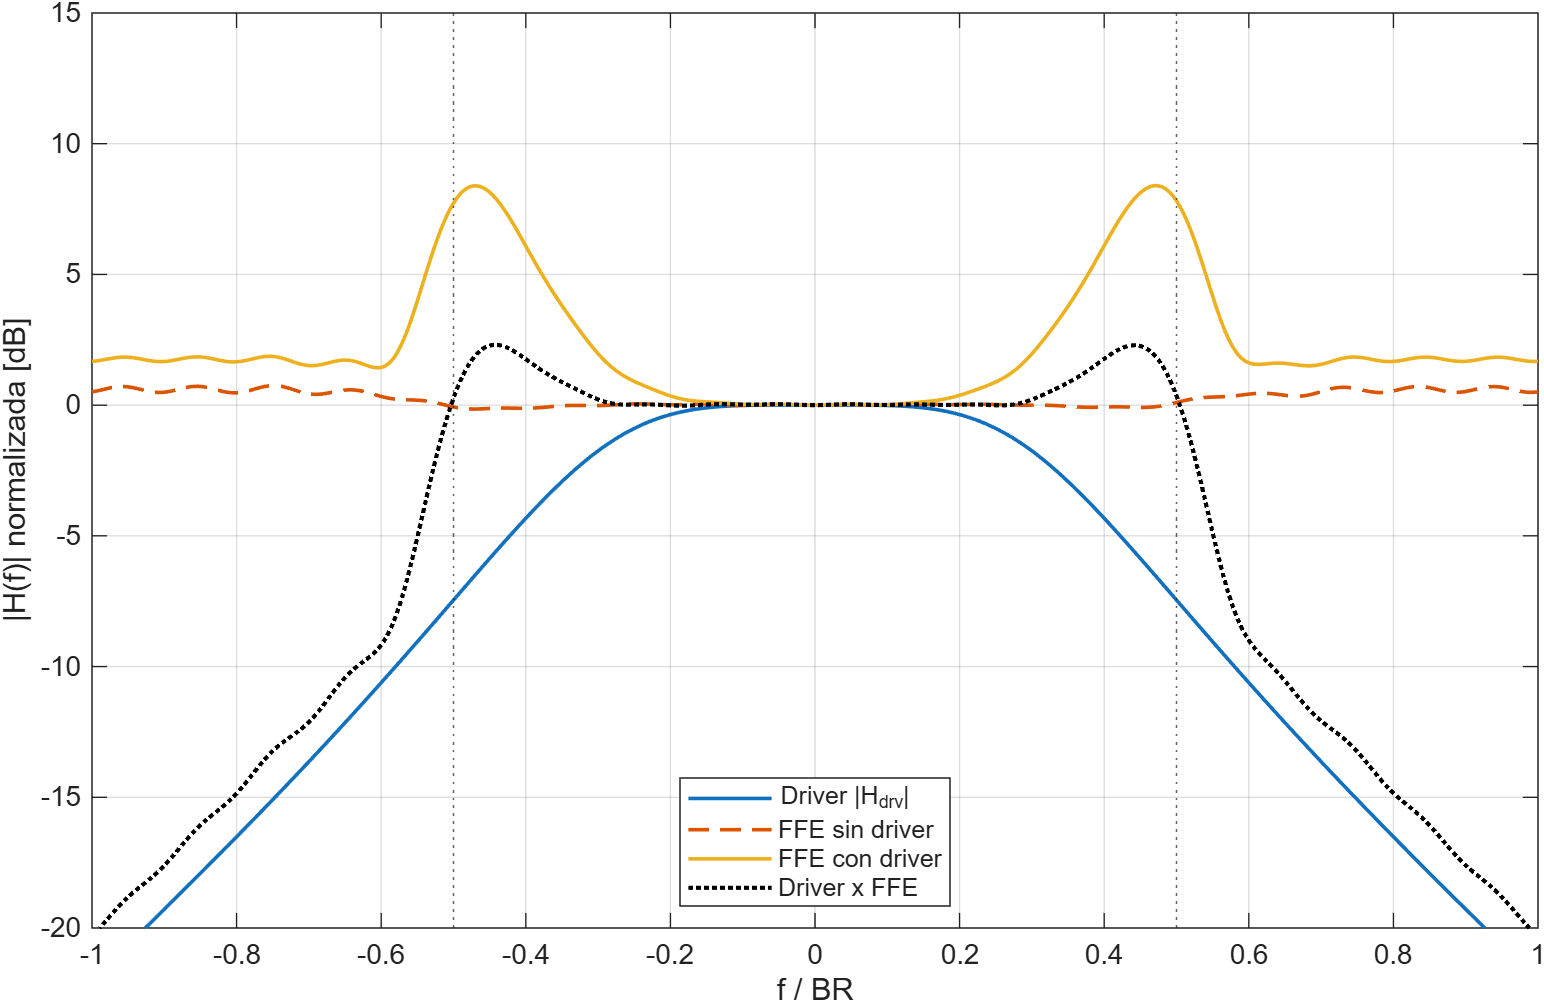
\includegraphics[width=0.8\textwidth]{figuras/ej2_ffe_driver.png}
\caption{Respuesta del driver, del FFE sin y con el driver, y del producto
driver por FFE ($E_b/N_0 = 16$~dB).}
\label{fig:ej2_drv}
\end{figure}

Sin el driver el FFE es plano. Con el driver, el FFE cambia su solución y
levanta $7.8$~dB en Nyquist, de modo que el producto queda plano en la
banda de la señal: compensa la distorsión lineal del driver. Fuera de la
banda de la señal ($|f| > 0.75\,BR$) no hay energía y el FFE no tiene
nada que ecualizar. El costo es la amplificación del ruido en las altas
frecuencias: la SNR en el slicer baja de $22.0$ a $20.2$~dB.

%==========================================================================
\subsection*{Ejercicio 3: Compensación de desbalance I/Q}
%==========================================================================

Se barrieron por separado el error de ganancia I/Q (de $0$ a $3$~dB) y el
desbalance de fase I/Q (de $0^\circ$ a $15^\circ$), con transmisor ideal
en todo lo demás y canal impulso. Para cada valor se midió la penalidad de
$E_b/N_0$ a $\mathrm{BER} = 10^{-2}$ y $10^{-3}$ respecto de la curva
teórica, con el compensador apagado (identidad) y encendido
(Figuras~\ref{fig:ej3_gain} y~\ref{fig:ej3_phase}).

\begin{figure}[H]
\centering
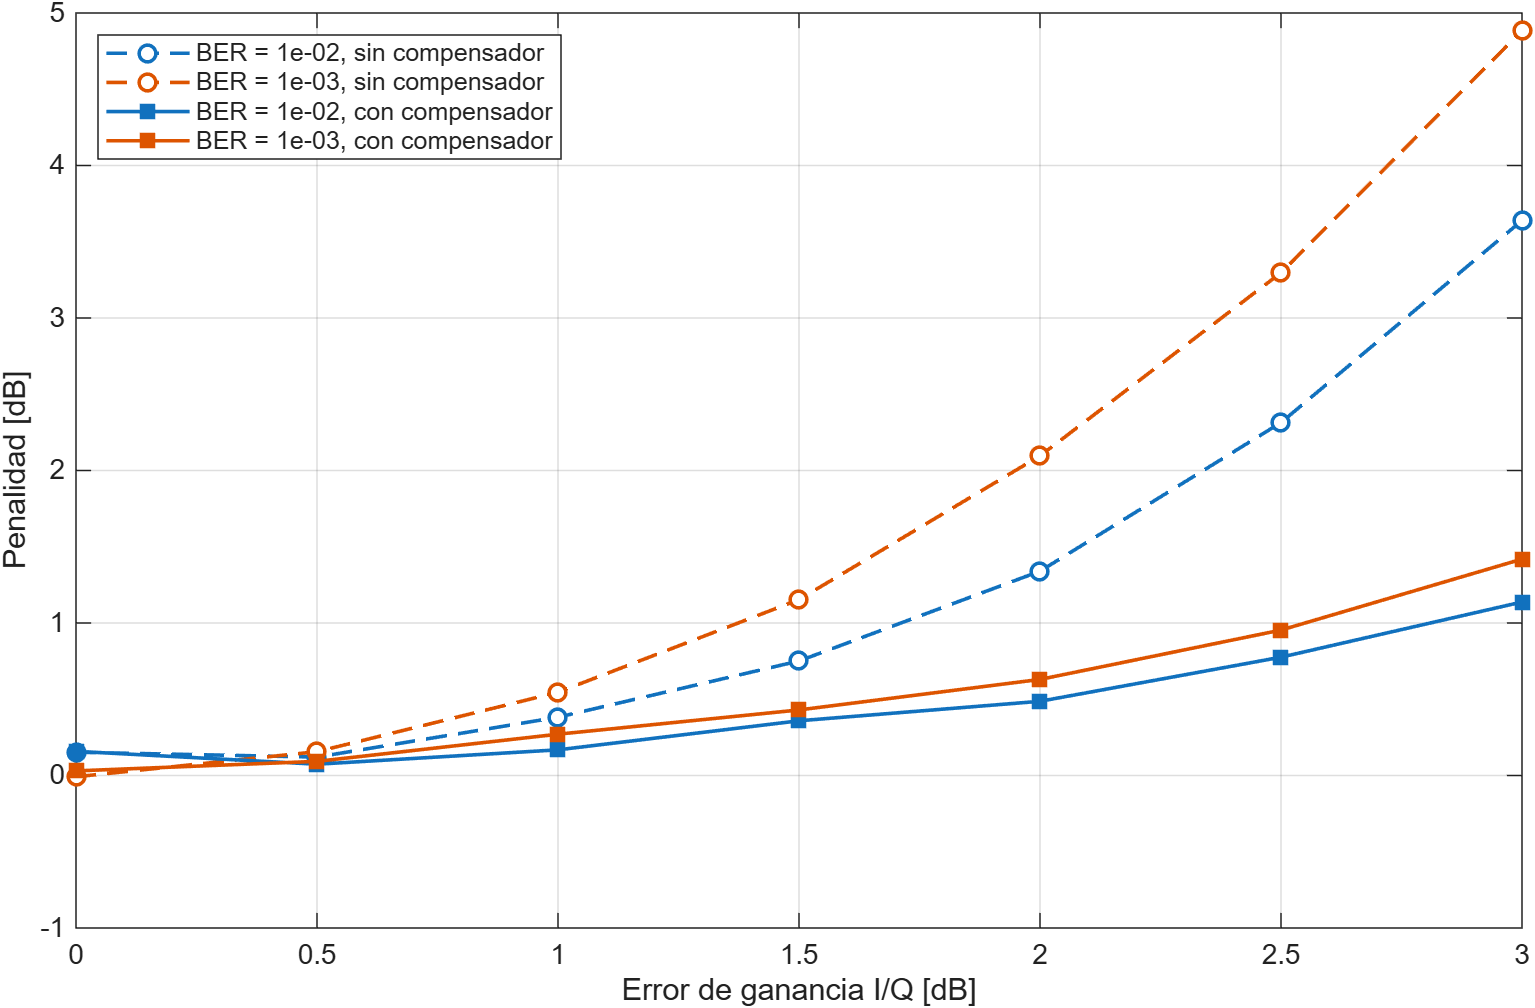
\includegraphics[width=0.75\textwidth]{figuras/ej3_pen_gain.png}
\caption{Penalidad en función del error de ganancia I/Q, sin y con el
compensador.}
\label{fig:ej3_gain}
\end{figure}

\begin{figure}[H]
\centering
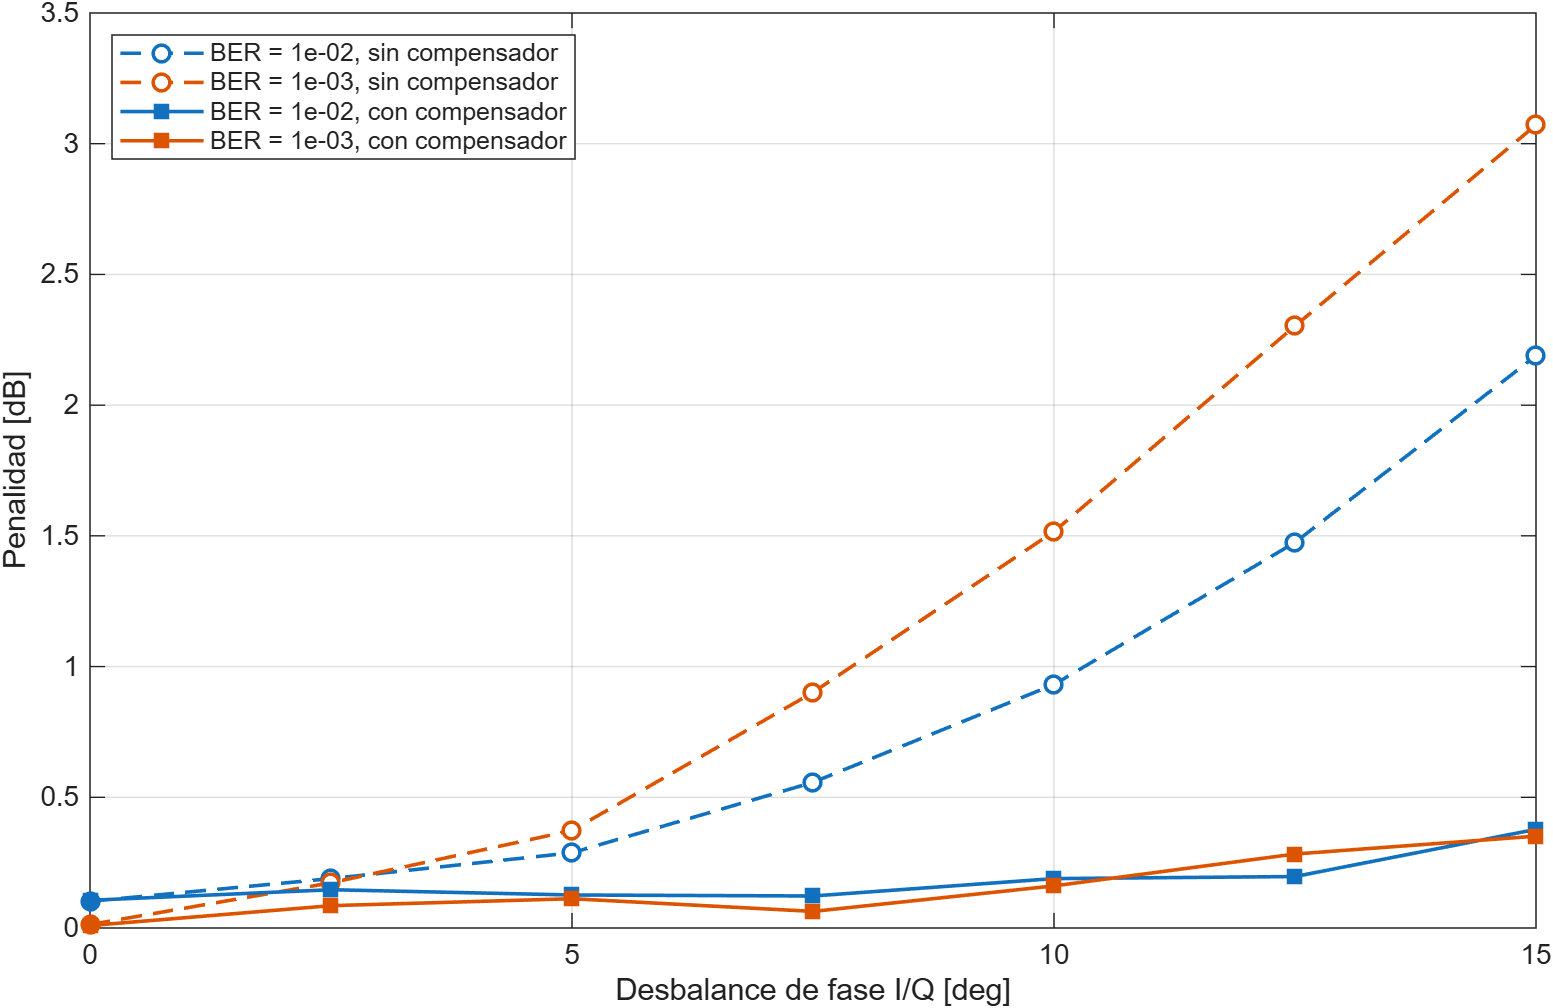
\includegraphics[width=0.75\textwidth]{figuras/ej3_pen_phase.png}
\caption{Penalidad en función del desbalance de fase I/Q, sin y con el
compensador.}
\label{fig:ej3_phase}
\end{figure}

\begin{table}[H]
\centering
\small
\begin{tabular}{lcccc}
\toprule
& \multicolumn{2}{c}{Sin compensador} & \multicolumn{2}{c}{Con compensador} \\
\cmidrule(lr){2-3}\cmidrule(lr){4-5}
Desperfecto & @ $10^{-2}$ & @ $10^{-3}$ & @ $10^{-2}$ & @ $10^{-3}$ \\
\midrule
Ganancia $1$~dB      & $0.38$ & $0.55$ & $0.17$ & $0.27$ \\
Ganancia $2$~dB      & $1.34$ & $2.10$ & $0.49$ & $0.63$ \\
Ganancia $3$~dB      & $3.64$ & $4.88$ & $1.14$ & $1.42$ \\
Fase $5^\circ$       & $0.29$ & $0.37$ & $0.13$ & $0.11$ \\
Fase $10^\circ$      & $0.93$ & $1.52$ & $0.19$ & $0.16$ \\
Fase $15^\circ$      & $2.19$ & $3.07$ & $0.38$ & $0.35$ \\
\bottomrule
\end{tabular}
\caption{Penalidad en dB para algunos valores de los barridos.}
\label{tab:ej3}
\end{table}

Sin compensación la penalidad crece rápidamente: el desbalance deforma la
constelación (un error de ganancia la estira en un eje y uno de fase la
inclina) y los puntos se acercan a los umbrales del slicer. La penalidad
es mayor a $\mathrm{BER} = 10^{-3}$, porque a menor BER los errores los
producen las colas del ruido, y cualquier acercamiento a los umbrales pesa
más.

Con el compensador la penalidad del desbalance de fase prácticamente
desaparece: queda por debajo de $0.4$~dB a $15^\circ$. La del error de
ganancia se reduce mucho, pero no a cero, y el residuo crece con el error
($1.4$~dB a $3$~dB de error). No es una limitación del compensador sino
una pérdida inherente: el ruido se suma en el canal, después del
desbalance. Con la potencia total fija, la lane más débil transmite menos
potencia que en el caso ideal y llega con peor relación señal a ruido.
El compensador iguala las amplitudes, pero al amplificar esa lane también
amplifica su ruido. Por ejemplo, con $3$~dB de error la lane I lleva
$10\log_{10}(3/2) = 1.76$~dB menos potencia que en el caso ideal y la Q,
$1.25$~dB más. La BER queda dominada por la lane débil, y la penalidad
residual ($1.1$ a $1.4$~dB) queda apenas por debajo de los $1.76$~dB que
pierde esa lane. Con el desbalance de fase pasa algo
similar pero mucho más chico: deshacer la mezcla entre lanes amplifica el
ruido en un factor $1/\cos\Delta\phi$, que a $15^\circ$ es de apenas
$0.3$~dB.

%==========================================================================
\subsection*{Ejercicio 4: Compensación de skew}
%==========================================================================

Se barrió el skew I/Q entre $-1$ y $1$~UI en pasos de $0.125$~UI, sin
compensador y con el compensador de 3, 7 y 15 taps por lane, midiendo la
penalidad a $\mathrm{BER} = 10^{-2}$ y $10^{-3}$
(Figuras~\ref{fig:ej4_2} y~\ref{fig:ej4_3}). Los puntos que faltan en las
curvas son aquellos en los que la BER objetivo no se alcanza ni con
$8$~dB de margen sobre el valor teórico.

\begin{figure}[H]
\centering
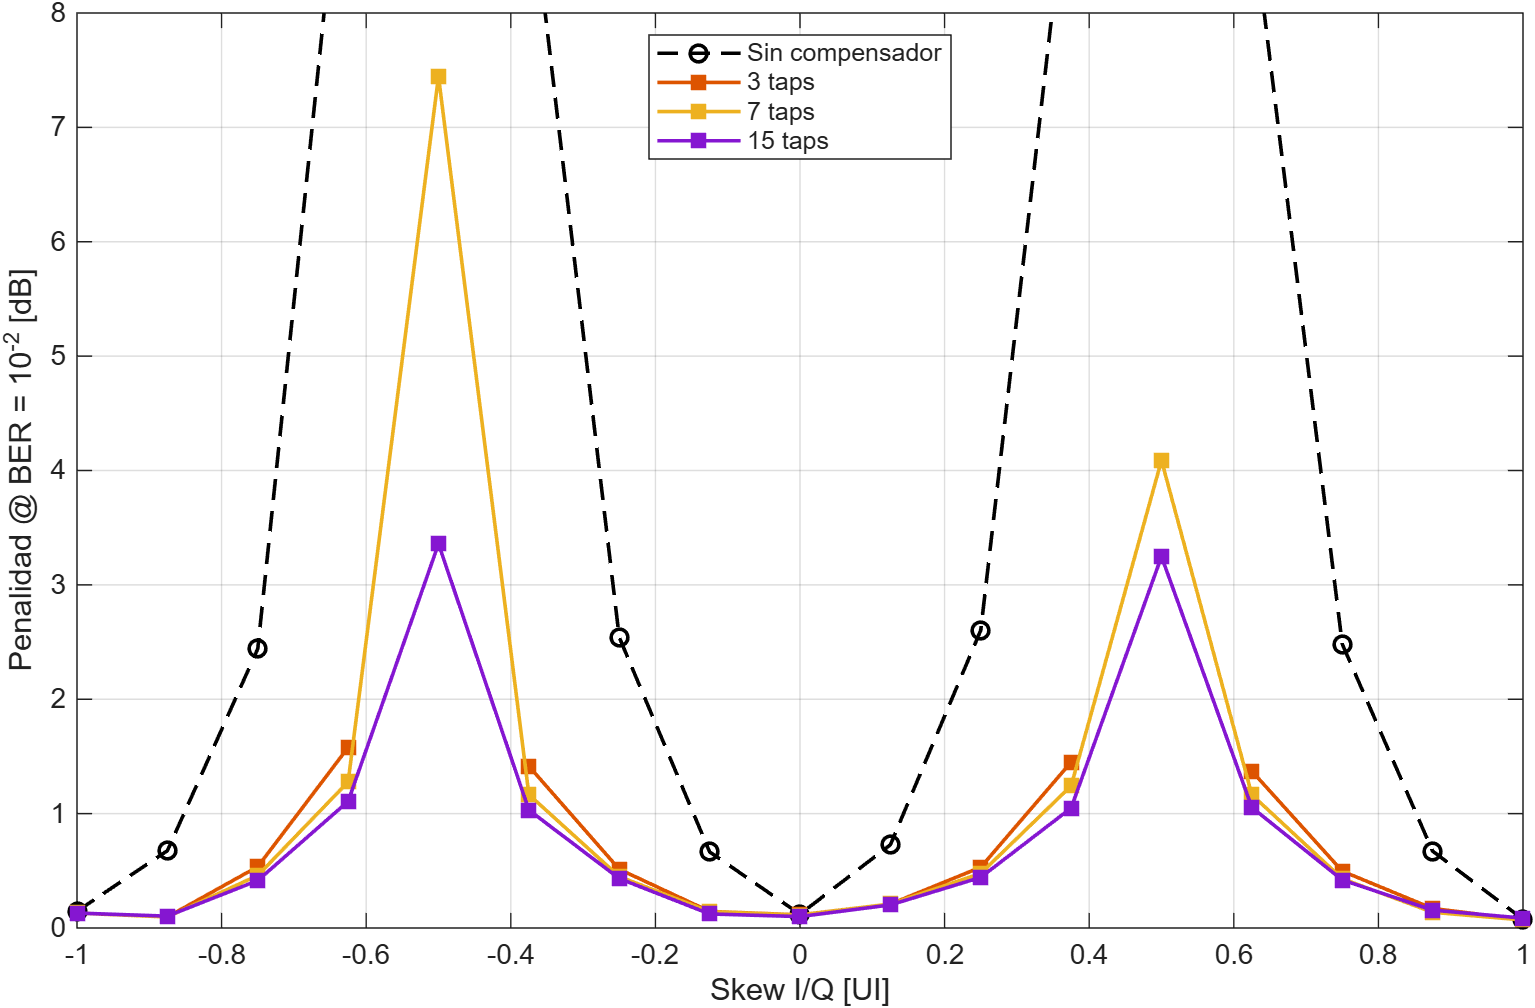
\includegraphics[width=0.75\textwidth]{figuras/ej4_pen_skew_2.png}
\caption{Penalidad a $\mathrm{BER} = 10^{-2}$ en función del skew I/Q.}
\label{fig:ej4_2}
\end{figure}

\begin{figure}[H]
\centering
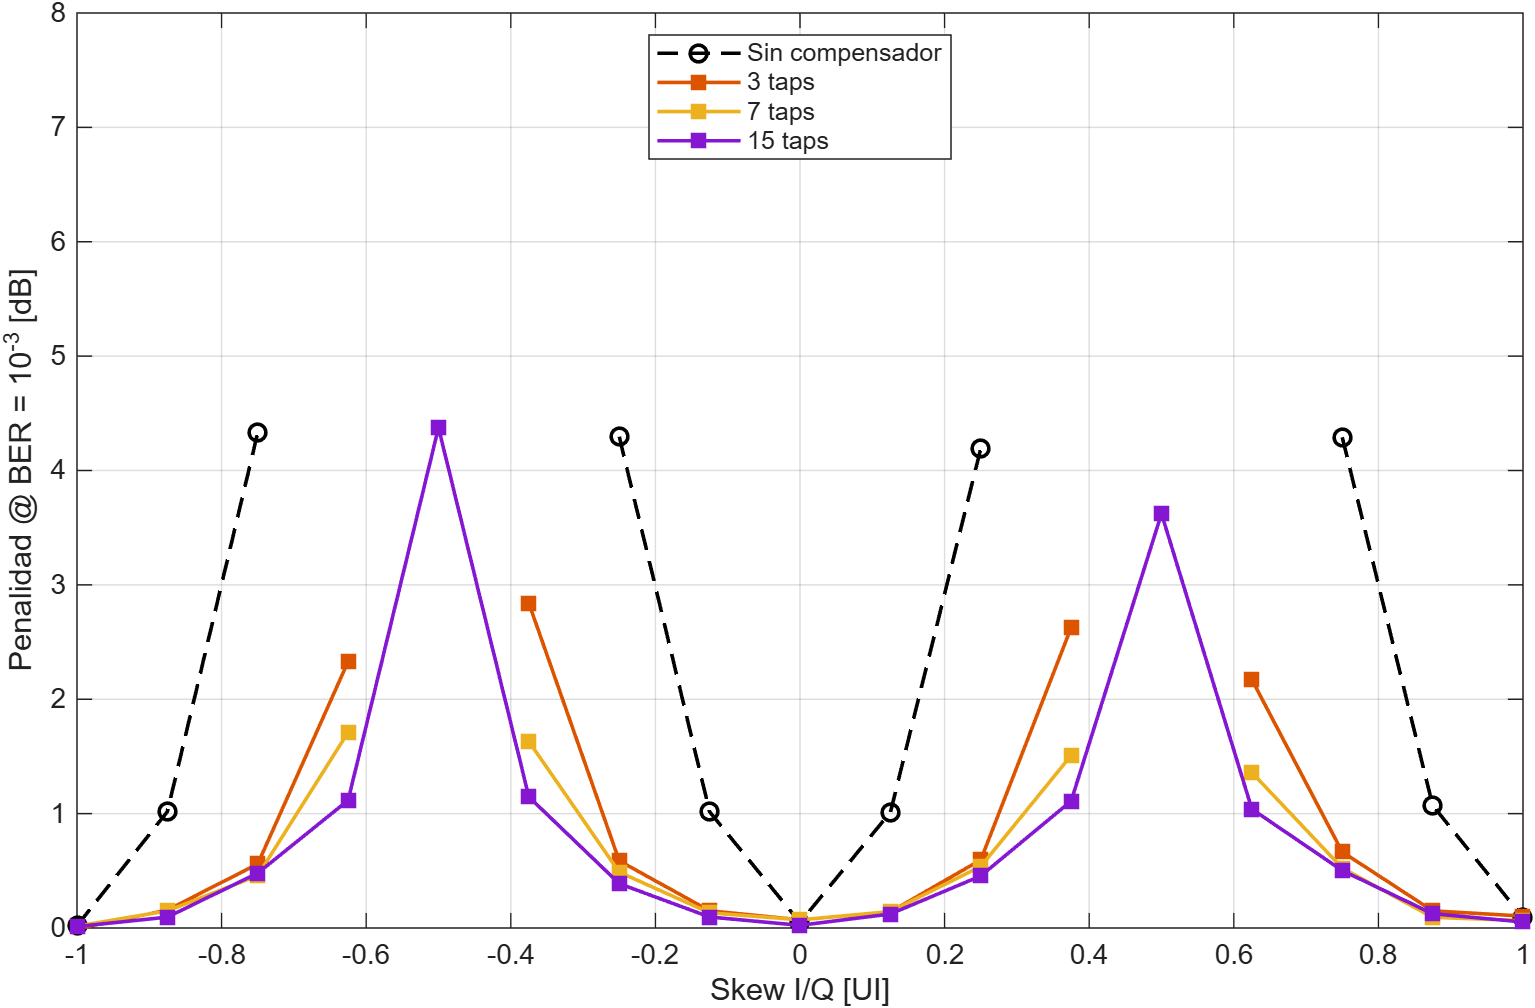
\includegraphics[width=0.75\textwidth]{figuras/ej4_pen_skew_3.png}
\caption{Penalidad a $\mathrm{BER} = 10^{-3}$ en función del skew I/Q.}
\label{fig:ej4_3}
\end{figure}

\begin{table}[H]
\centering
\small
\begin{tabular}{lccccc}
\toprule
Skew [UI] & $0.125$ & $0.25$ & $0.375$ & $0.5$ & $1$ \\
\midrule
Sin compensador & $1.01$ & $4.19$ & --- & --- & $0.09$ \\
3 taps          & $0.14$ & $0.60$ & $2.63$ & --- & $0.10$ \\
7 taps          & $0.14$ & $0.54$ & $1.51$ & --- & $0.06$ \\
15 taps         & $0.12$ & $0.46$ & $1.11$ & $3.62$ & $0.05$ \\
\bottomrule
\end{tabular}
\caption{Penalidad en dB a $\mathrm{BER} = 10^{-3}$ para skew positivo
(``---'': no se alcanza la BER objetivo).}
\label{tab:ej4}
\end{table}

Las curvas son simétricas respecto de cero y periódicas en un UI. Sin
compensador, ya con $0.25$~UI la penalidad supera los $4$~dB y entre
$0.375$ y $0.625$~UI el sistema no alcanza la BER objetivo. En cambio, con
skew de exactamente $\pm1$~UI la penalidad vuelve a ser nula: la lane Q
llega desplazada un símbolo entero, el receptor arma puntos válidos con
$I(n)$ y $Q(n-1)$ y la alineación 2 por lane lo corrige sin necesidad de
ningún filtro.

Con el compensador la penalidad se reduce en todo el rango. Para skew de
hasta $0.25$~UI queda por debajo de $0.6$~dB con cualquier cantidad de
taps; a medida que el skew se acerca a $0.5$~UI hacen falta más taps,
porque el FIR tiene que interpolar la lane retrasada a mitad de camino
entre dos símbolos, y esa interpolación necesita una respuesta más larga.
A $0.375$~UI la penalidad baja de $2.6$~dB con 3 taps a $1.1$~dB con 15.

El peor caso es $\pm0.5$~UI. Solo el compensador de 15 taps alcanza la
BER objetivo, con unos $3.6$~dB de penalidad. Ahí la lane retrasada se
muestrea exactamente entre dos símbolos: el ojo está cerrado antes de la
compensación, y el compensador, que opera a un símbolo por muestra, tiene
que reconstruir la señal en un punto donde las muestras de los dos
símbolos vecinos pesan lo mismo. Es una limitación del propio esquema y
no de la adaptación: con los coeficientes óptimos calculados con los
símbolos verdaderos ($E_b/N_0 = 16$~dB, SNR ideal de $22.0$~dB), a
$0.5$~UI el compensador llega a $17.6$, $18.7$ y $19.1$~dB con 7, 15 y 31
taps, es decir, entre $3$ y $4.5$~dB por debajo del ideal, en línea con la
penalidad medida. Un compensador que operara a dos muestras por símbolo,
antes del FFE, debería reducir esta limitación.

%==========================================================================
\subsection*{Ejercicio 5: Sistema completo}
%==========================================================================

Se simularon todos los efectos a la vez (Tabla~\ref{tab:ej5_cfg}) para
verificar que la cadena de compensación funciona en conjunto y que la
duración de las etapas de la máquina de estados es suficiente.

\begin{table}[H]
\centering
\small
\begin{tabular}{ll}
\toprule
Bloque & Configuración \\
\midrule
Driver  & $G = 15$~dB, $f_n = 2BR/3$, $\zeta = 0.25$, ruido $10$~mV, Rapp $p = 2$, $V_{sat} = 3$~V \\
MZM     & $V_\pi = 5$~V, $2.8$~V$_{pp}$ de excitación, pérdidas $3$, $3$ y $4$~dB, respuesta del MZM \\
Láser   & ideal \\
LTX     & error de ganancia $1$~dB, desbalance de fase $5^\circ$, skew $0.3$~UI \\
Canal   & pasabajos con corte en $0.5\,BR$, $E_b/N_0 = 18$~dB \\
Portadora & fase $0.7$~rad, offset $BR/200$, jitter de $0.05$~rad a $10^{-4}\,BR$ \\
\bottomrule
\end{tabular}
\caption{Configuración del sistema completo.}
\label{tab:ej5_cfg}
\end{table}

\begin{table}[H]
\centering
\small
\begin{tabular}{lcc}
\toprule
& BER & SNR en el slicer \\
\midrule
Con los compensadores del LTX & $5.3\times10^{-5}$ & $19.9$~dB \\
Sin los compensadores del LTX & $7.5\times10^{-2}$ & $10.2$~dB \\
\bottomrule
\end{tabular}
\caption{Resultado del sistema completo.}
\label{tab:ej5_res}
\end{table}

La Figura~\ref{fig:ej5_const} muestra la constelación a la entrada del
slicer en cada etapa y la Tabla~\ref{tab:ej5_snr}, la SNR al final de
cada una. En las etapas 1 a 3 el FFE converge y la recuperación de
portadora engancha; las etapas 4 a 6 terminan de ajustar el lazo
principal. La constelación sigue mostrando una dispersión horizontal, que
es el efecto del skew y del desbalance: ningún algoritmo del lazo
principal puede corregirlos. La etapa 7 corrige el desbalance y la 8, el
skew, que es la que más aporta ($14.1 \rightarrow 19.9$~dB). No hubo
cycle slips, y el offset residual que deja el RFD queda absorbido por la
rama integral del DPLL fino.

En la Figura~\ref{fig:ej5_coef} se ve que el compensador de skew corrige
la lane I y deja la Q prácticamente en un impulso, aunque el skew se
aplicó a la Q en el transmisor. Como el skew es relativo, lo que importa
es cuál de las lanes quedó desalineada respecto de la temporización que
eligió el FFE: en esta corrida el FFE se alineó con la lane Q, y desde el
receptor la lane desplazada es la I.

\begin{table}[H]
\centering
\small
\begin{tabular}{lc}
\toprule
Etapa & SNR [dB] \\
\midrule
1: FFE-CMA            & 11.4 \\
2: FFE-CMA + RFD      & 11.3 \\
3: + FCR 4ª potencia  & 12.0 \\
4: FFE-CMA + FCR-DD   & 13.0 \\
5: FFE-DD + FCR-DD    & 13.7 \\
6: Alineación + CS    & 13.9 \\
7: Desbalance I/Q     & 14.1 \\
8: Skew               & 19.9 \\
9: Alineación 2       & 20.0 \\
10: BER               & 19.8 \\
\bottomrule
\end{tabular}
\caption{SNR al final de cada etapa (error contra las propias decisiones,
últimos 5000 símbolos).}
\label{tab:ej5_snr}
\end{table}

\begin{figure}[H]
\centering
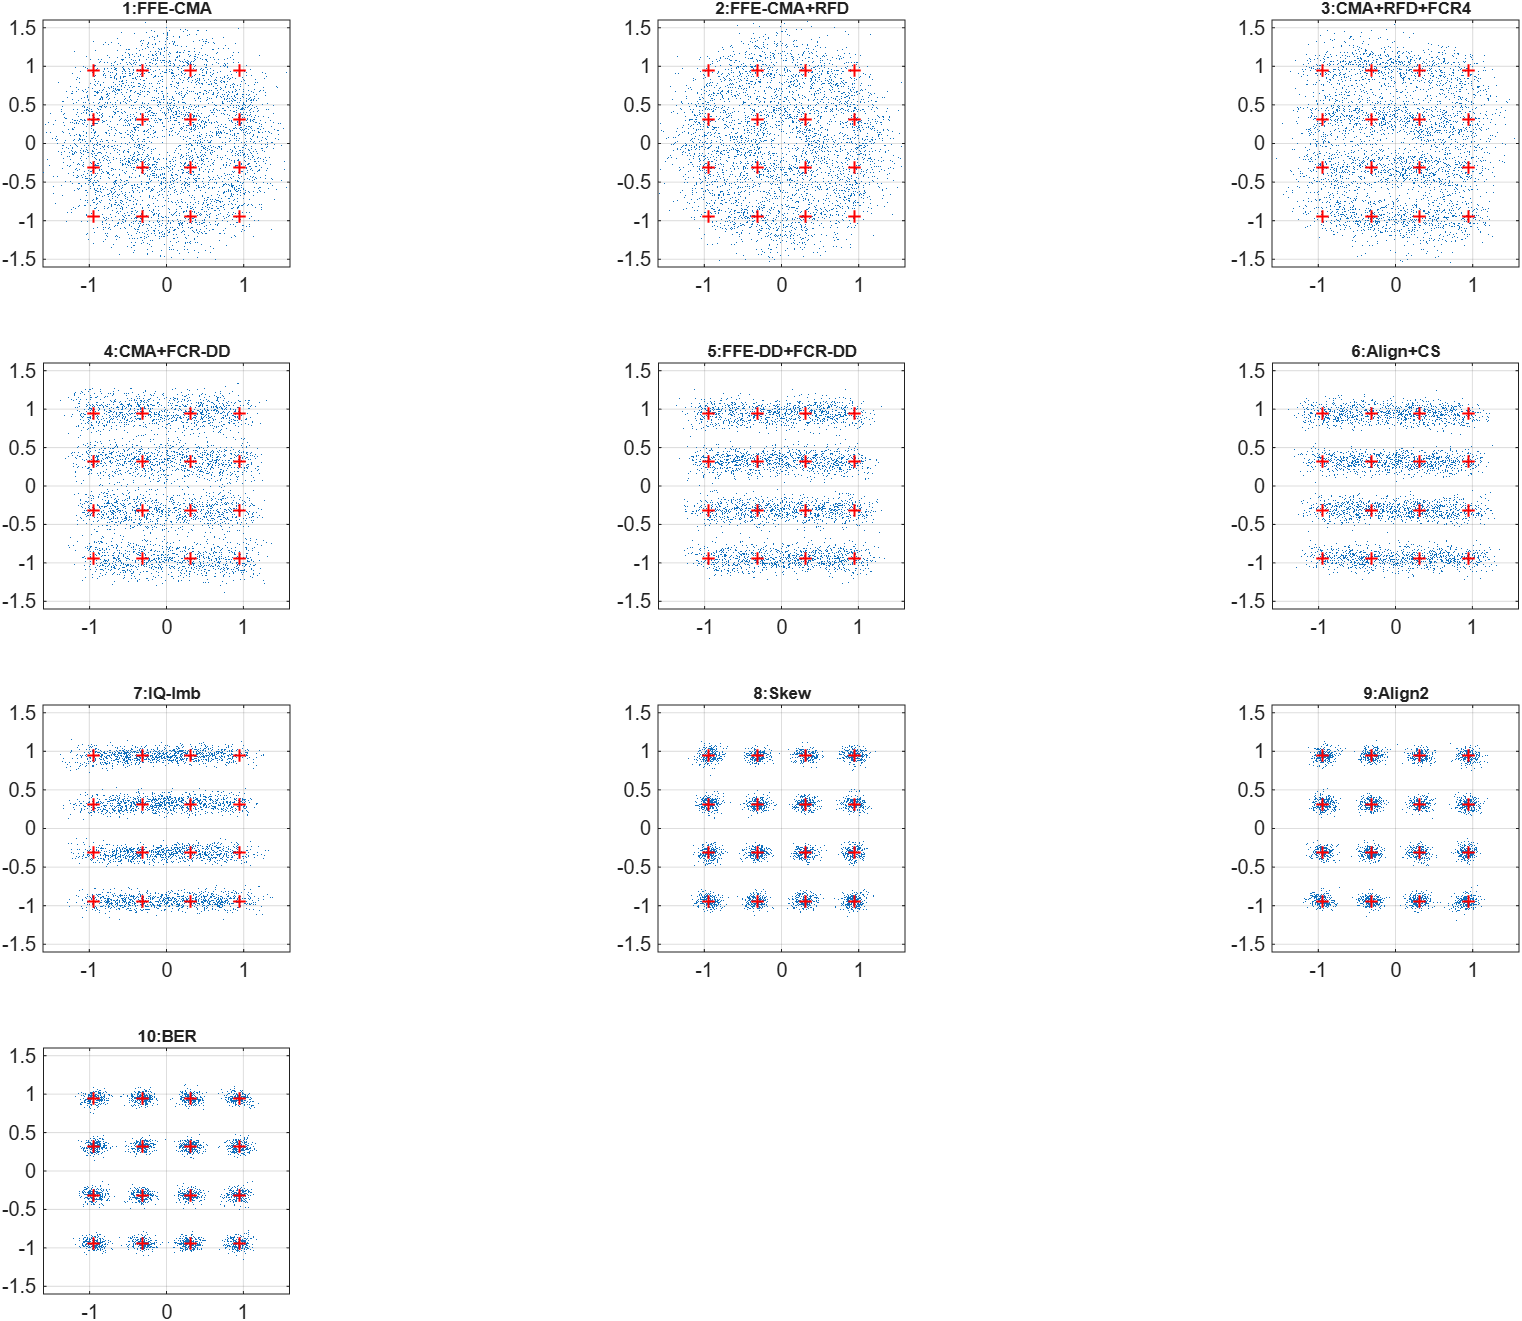
\includegraphics[width=\textwidth]{figuras/ej5_constelaciones.png}
\caption{Constelación a la entrada del slicer en cada etapa de la máquina
de estados. Desde la etapa 7 se muestra la salida de los compensadores.}
\label{fig:ej5_const}
\end{figure}

\begin{figure}[H]
\centering
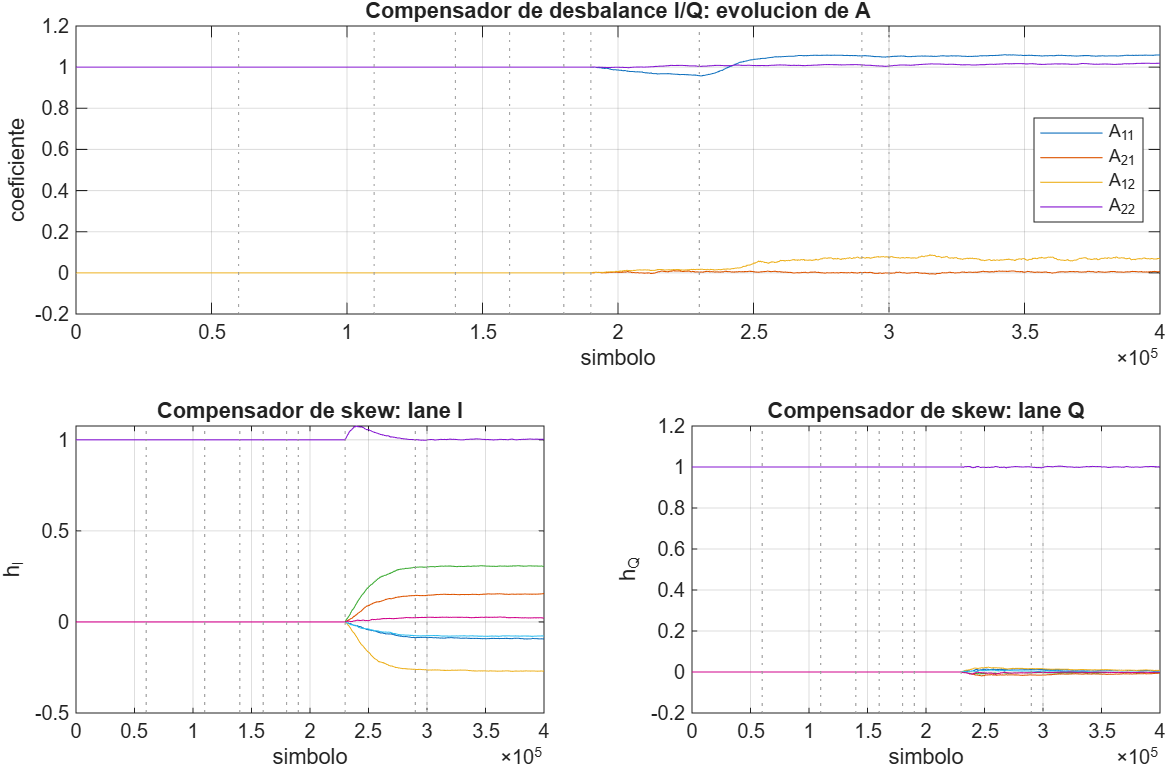
\includegraphics[width=\textwidth]{figuras/ej5_ltx_coef.png}
\caption{Evolución de los coeficientes de los compensadores de desbalance
I/Q y de skew.}
\label{fig:ej5_coef}
\end{figure}

\begin{figure}[H]
\centering
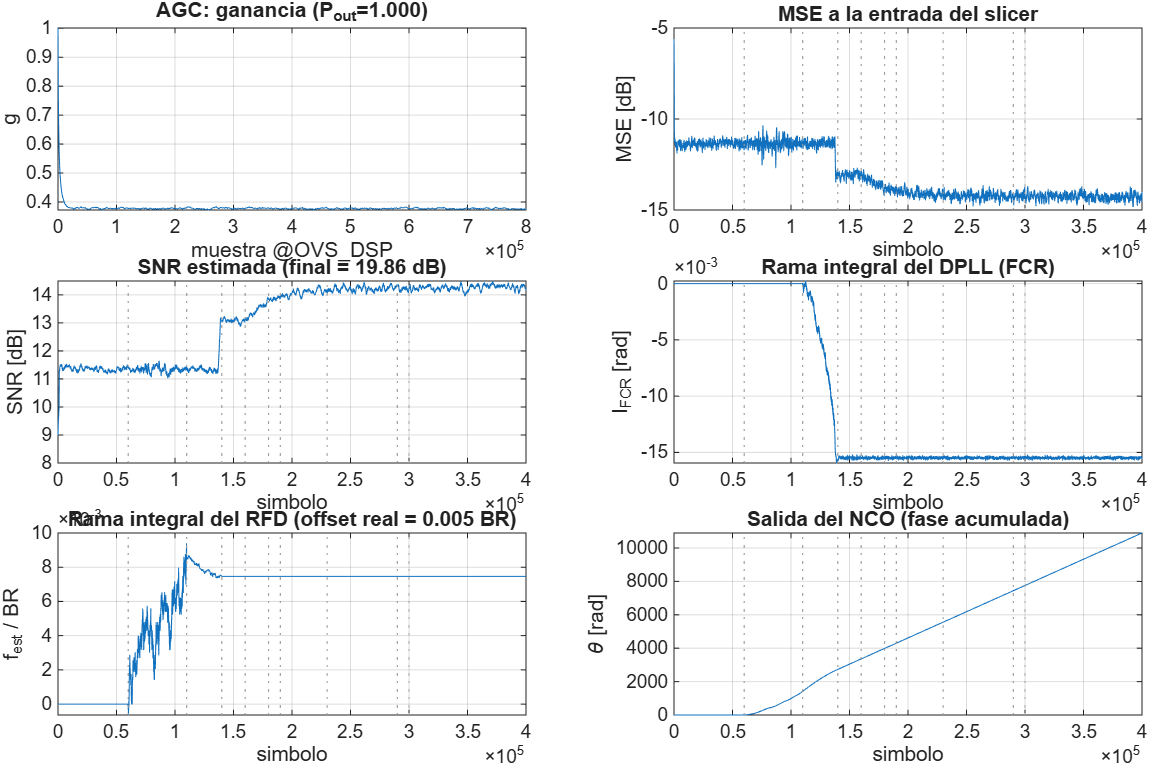
\includegraphics[width=\textwidth]{figuras/ej5_metricas.png}
\caption{AGC, MSE, SNR estimada, ramas integrales del FCR y del RFD y
salida del NCO. Las líneas punteadas marcan las transiciones de la máquina
de estados.}
\label{fig:ej5_met}
\end{figure}

Para que la adquisición sea robusta fue necesario acotar la limitación de
ancho de banda. Con el corte en $0.4\,BR$, la interferencia entre
símbolos junto con el skew sesga la estimación del RFD, el residuo supera
el rango de enganche del DPLL y aparecen cycle slips. Con $0.5\,BR$ el
sistema engancha en todas las semillas probadas. Además, la relación de
extinción del MZM se dejó infinita: con un valor finito la portadora no
se suprime por completo y aparece un nivel de continua en la
constelación, que ninguno de los bloques del receptor compensa. Con
$ER = 25$~dB, en una corrida de prueba con el MZM real y sin el resto de
los desperfectos ($E_b/N_0 = 20$~dB), ese nivel es el 8~\% del radio de la
constelación y la SNR en el slicer cae de $26.0$ a $13.8$~dB.

%==========================================================================
\subsection*{Ejercicio 6: Preguntas analíticas}
%==========================================================================

\paragraph{¿Por qué los ecualizadores de I/Q y de skew no utilizan leakage?}
En el FFE el leakage hace falta porque está muestreado a dos muestras por
símbolo y la señal no tiene energía fuera de su banda: hay combinaciones
de coeficientes que no cambian la salida, y el ruido de gradiente las
hace crecer sin límite. El leakage las mantiene acotadas. Los
compensadores del LTX operan a un símbolo por muestra, donde la señal
ocupa toda la banda: la solución es única y los coeficientes no derivan.
Agregar leakage solo tiraría los coeficientes hacia cero, lo que en estos
bloques es justamente un error de ganancia: introduciría la misma clase
de desperfecto que se quiere corregir.

\paragraph{¿Por qué el desbalance de I/Q puede compensarse con un solo tap?}
Porque es un efecto sin memoria: el error de ganancia y el de fase
dependen solo de la muestra actual de cada lane, no de las anteriores ni
de las siguientes. La salida en el instante $n$ es una combinación lineal
de $I(n)$ y $Q(n)$, y se invierte con una matriz de $2\times2$ aplicada
muestra a muestra.

\paragraph{¿Por qué el compensador de skew no posee filtros cruzados?}
Porque el skew es un retardo de una lane respecto de la otra y no mezcla
I con Q: cada lane necesita solo su propio filtro de interpolación. Se
verificó con la solución óptima calculada con los símbolos verdaderos: a
$0.5$~UI de skew, agregar filtros cruzados mejora la SNR en menos de
$0.05$~dB con 7, 15 o 31 taps.

\paragraph{¿Por qué el filtro FFE no puede compensar estos impairments?}
El FFE es un único filtro complejo que se aplica a la señal $I + jQ$:
trata a las dos lanes de la misma manera, con la misma ganancia y el
mismo retardo. El desbalance de ganancia o de fase y el skew son
justamente diferencias entre las lanes: requieren aplicar a $Q$ algo
distinto que a $I$, y un filtro complejo no puede hacerlo. Visto de otra
forma, estos desperfectos agregan a la señal una componente proporcional
a su conjugada, $\alpha\,x + \beta\,x^*$, y un filtro lineal sobre $x$ no
puede generar ni cancelar términos en $x^*$.

Un ecualizador que sí podría compensarlos es uno que procese por separado
las lanes: un FFE de $2\times2$ real (filtros $I\!\rightarrow\!I$,
$Q\!\rightarrow\!I$, $I\!\rightarrow\!Q$ y $Q\!\rightarrow\!Q$),
equivalente a filtrar en paralelo la señal y su conjugada,
$y = \mathbf{w}_1^H \mathbf{r} + \mathbf{w}_2^H \mathbf{r}^*$. Operando a
dos muestras por símbolo, corregiría en un solo bloque la ISI del canal,
el desbalance de ganancia y fase y el skew, incluso fraccionario.

\paragraph{Distorsión del driver.}
Se habilitó la no linealidad de Rapp del driver ($p = 2$) y se barrió la
tensión de saturación $V_{sat}$ con la excitación fija. Para aislar el
efecto de la no linealidad, el MZM se dejó lineal y la respuesta en
frecuencia del driver plana en la banda de la señal. Sin saturación, la
señal a la salida del driver tiene un pico de $1.09$~V, de modo que el eje
de la Figura~\ref{fig:ej6_pen} indica cuánto supera ese pico a $V_{sat}$.

\begin{figure}[H]
\centering
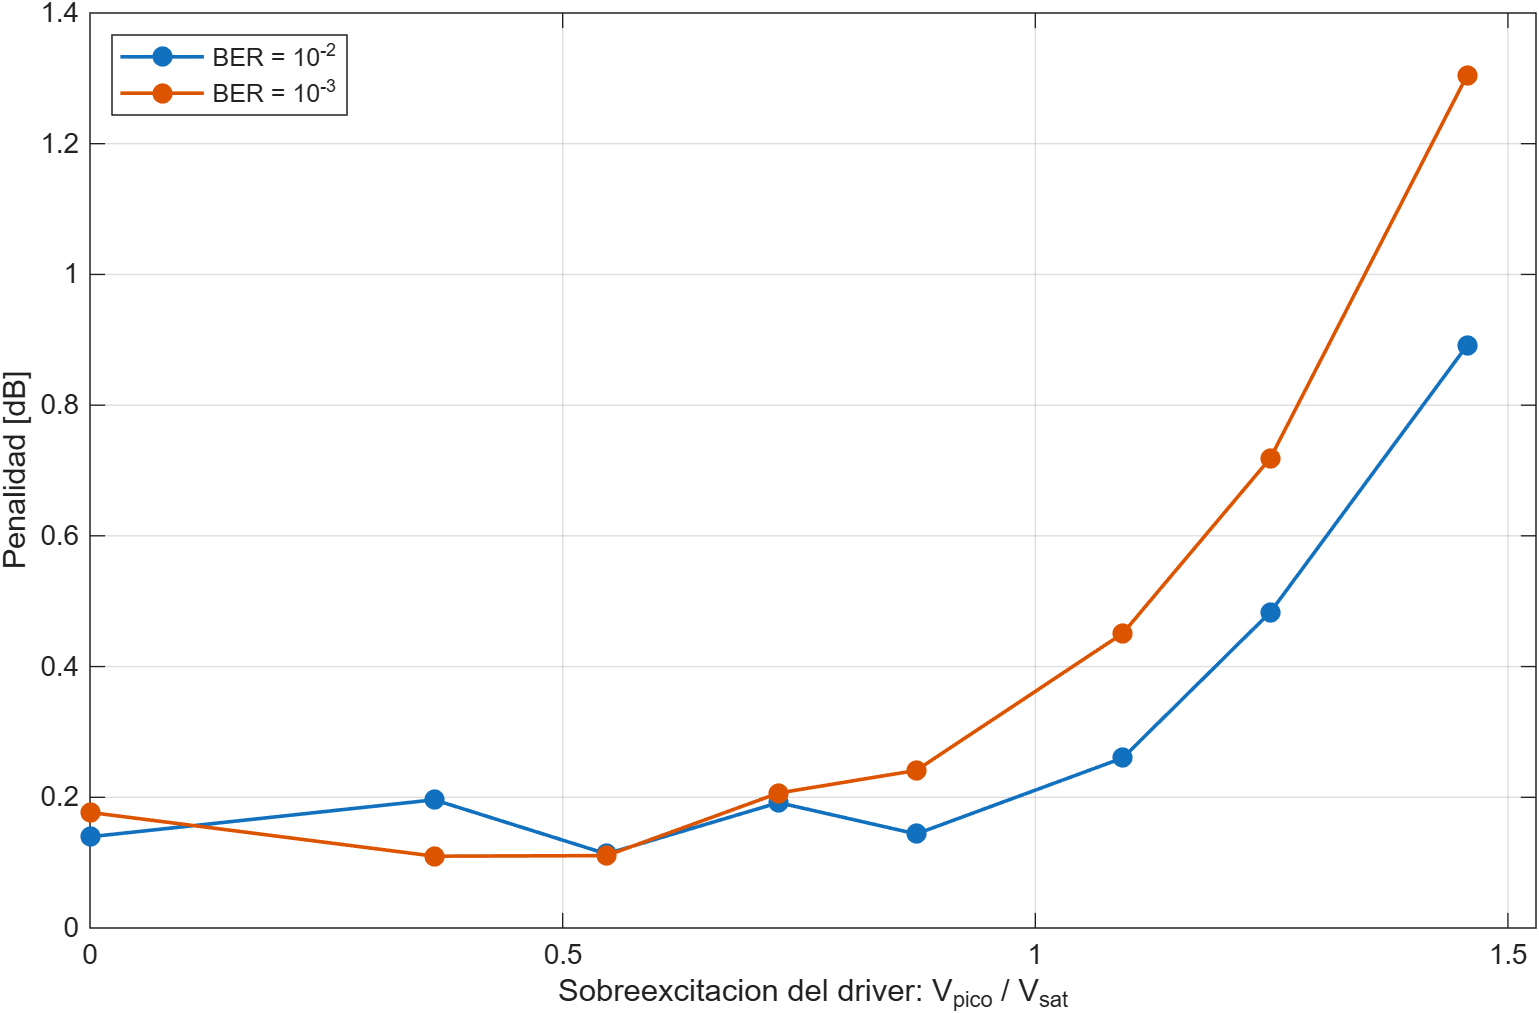
\includegraphics[width=0.7\textwidth]{figuras/ej6_pen_vsat.png}
\caption{Penalidad en función de la sobreexcitación del driver
($V_{pico}/V_{sat}$; el punto en cero corresponde al driver sin no
linealidad).}
\label{fig:ej6_pen}
\end{figure}

Mientras $V_{sat}$ está por encima del pico de la señal, la penalidad no
cambia (alrededor de $0.15$~dB). Cuando la señal empieza a entrar en
saturación la degradación crece rápidamente: $0.45$~dB con
$V_{sat} = 1$~V, $0.72$~dB con $0.875$~V y $1.3$~dB con $0.75$~V, a
$\mathrm{BER} = 10^{-3}$. Con $E_b/N_0 = 30$~dB, donde el ruido del canal
deja de enmascararla, la SNR en el slicer cae de $35.4$~dB sin distorsión
a $23.1$~dB con $V_{sat} = 0.75$~V.

\begin{figure}[H]
\centering
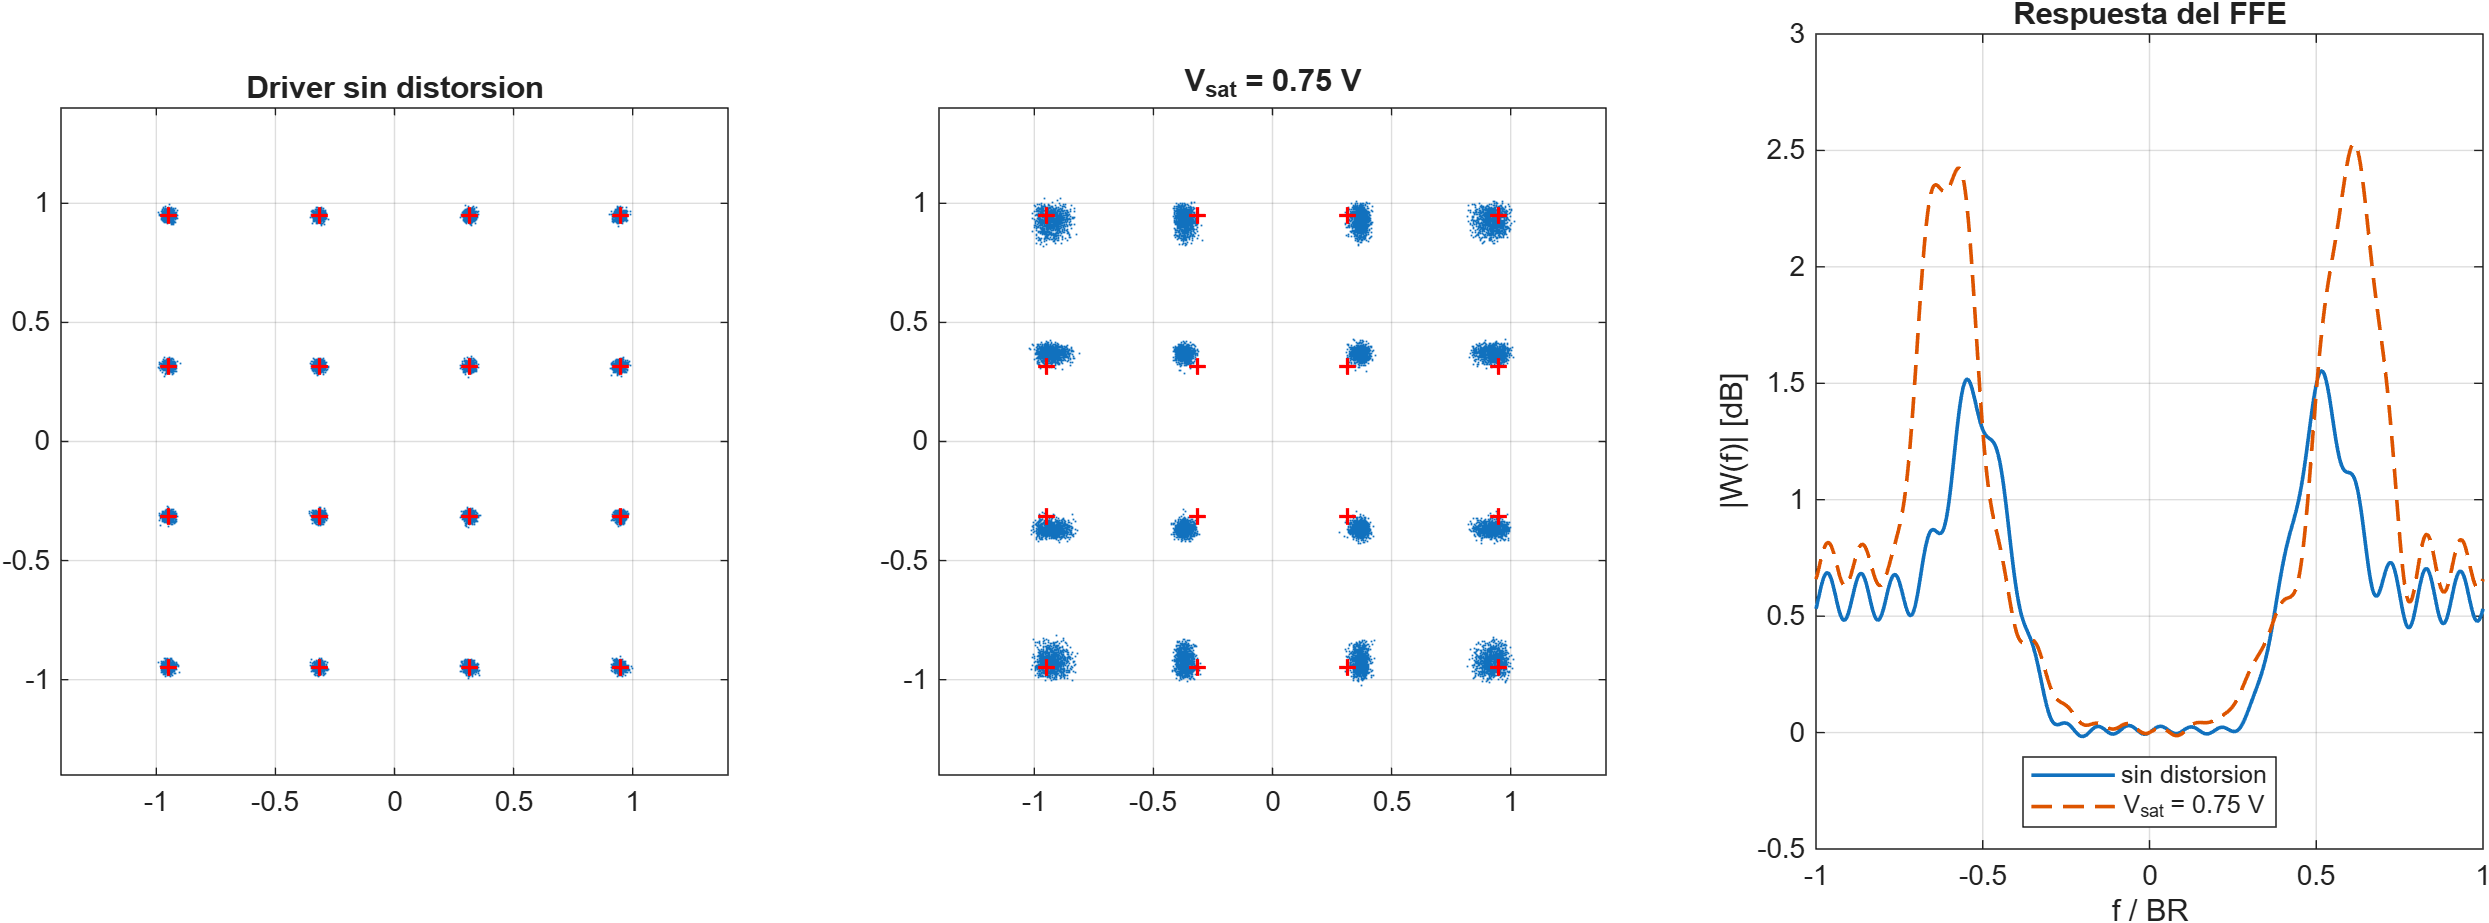
\includegraphics[width=\textwidth]{figuras/ej6_constelacion_ffe.png}
\caption{Constelación a la entrada del slicer sin distorsión y con
$V_{sat} = 0.75$~V, y respuesta del FFE en ambos casos
($E_b/N_0 = 30$~dB).}
\label{fig:ej6_const}
\end{figure}

La Figura~\ref{fig:ej6_const} muestra por qué el FFE no puede hacer nada.
La saturación comprime más las amplitudes grandes que las chicas: los
niveles de la constelación dejan de estar equiespaciados (una vez
normalizada la potencia, los puntos internos quedan corridos hacia
afuera) y, como la compresión actúa sobre la forma de onda conformada,
aparecen nubes alrededor de cada punto. El FFE es un filtro lineal:
puede cambiar la respuesta en frecuencia o la escala de toda la señal,
pero aplica la misma ganancia a una amplitud grande que a una chica, así
que no puede devolverles el espaciado original. Su respuesta cambia poco
respecto del caso sin distorsión (levanta alrededor de $1$~dB más las
altas frecuencias, donde la saturación ensancha el espectro), y eso no
corrige la compresión. Compensar este efecto requiere
un bloque no lineal, como una predistorsión en el transmisor que aplique
la inversa de la curva del driver, o reducir la excitación para operar en
la zona lineal, a costa de relación señal a ruido.

%==========================================================================
\subsection*{Conclusiones}
%==========================================================================

Se integró el transmisor óptico de doble polarización al simulador del
trabajo práctico 1 y se agregaron los compensadores de desbalance I/Q y de
skew, con una máquina de estados de diez etapas. Con todos los bloques
nuevos apagados el simulador reproduce exactamente los resultados del
trabajo práctico 1, y con todos encendidos sobre un transmisor ideal la
penalidad respecto de la curva teórica queda por debajo de $0.1$~dB, una
vez corregido el sesgo MMSE de los ecualizadores dirigidos por decisiones.

El desbalance I/Q y el skew son diferencias entre las lanes I y Q, y por
eso el FFE, que trata a las dos lanes por igual, no puede corregirlos:
hacen falta bloques que procesen cada lane por separado. El compensador de
desbalance, de un solo tap, elimina prácticamente toda la penalidad del
desbalance de fase. Con el error de ganancia queda un residuo que no
depende del compensador: el ruido se suma después del desbalance y la lane
más débil llega con peor relación señal a ruido.

El compensador de skew reduce la penalidad en todo el rango, y más taps
permiten compensar skews mayores. Dos casos requirieron cuidado. Con
skew de un UI o más, el desfasaje entero entre lanes no produce error
detectable por decisiones y se resolvió con una alineación por lane. Cerca
de $0.5$~UI el ojo está cerrado y la adaptación dirigida por decisiones no
arranca, lo que obligó a un arranque ciego; aun así ese es el peor caso,
y la penalidad que queda es propia de compensar a un símbolo por muestra.

La simulación del sistema completo mostró que la cadena funciona en
conjunto: cada etapa de la máquina de estados mejora la señal y los
compensadores del LTX, encendidos con el lazo principal ya convergido,
llevan la SNR de $10.2$ a $19.9$~dB. También mostró que la adquisición
depende de la severidad del canal: con una limitación de ancho de banda
fuerte junto con skew, el detector de frecuencia gruesa se sesga y
aparecen cycle slips.

Por último, la no linealidad del driver no puede compensarse con ninguno
de los ecualizadores lineales del receptor: comprime los niveles de la
constelación de forma desigual. Para operar cerca de la saturación hace
falta una predistorsión en el transmisor; de lo contrario, la excitación
debe mantenerse en la zona lineal.
